\chapter{We need precision in thought and action to win arguments}
\label{chap:logicandproofs}


\begin{figure}[ht]
\centerline{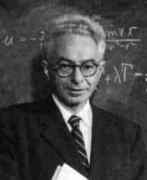
\includegraphics[width=1.0in]{images/courant.jpg}}
\caption*{\small ``Mathematics as an expression of the human mind reflects the active will, the contemplative reason, and the desire for aesthetic perfection. Its basic elements are logic and intuition, analysis and construction, generality and individuality.'' -- Richard Courant}
\end{figure}

\begin{figure}[ht]
\centerline{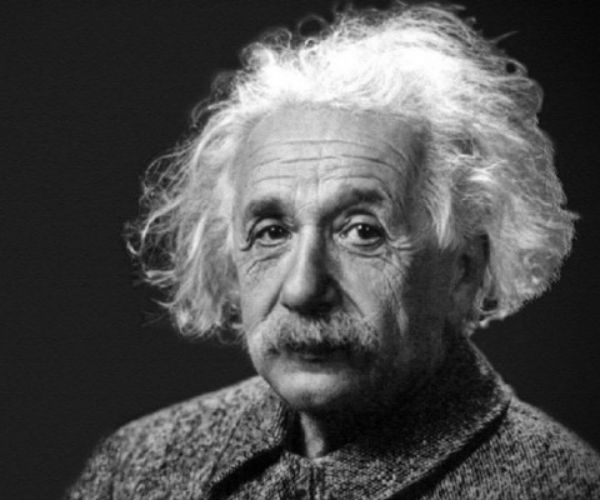
\includegraphics[width=1.0in]{images/einstein.jpeg}}
\caption*{\small ``Pure mathematics is, in its way, the poetry of logical ideas.'' -- Albert Einstein}
\end{figure}


Logic is the language of reasoning. Whenever we argue in mathematics, 
make a claim in science, or even decide something in everyday life, 
we  implicitly use the rules of logic. Boolean logic, named after the mathematician \href{https://en.wikipedia.org/wiki/George\_Boole}{George Boole}, 
provides a precise mathematical framework to study truth and falsity. 

In this chapter, we will introduce the basic building blocks of logic, 
learn how to represent them with truth tables, explore important rules like De Morgan’s laws, 
understand how to work with more than two statements at a time, 
and examine subtle but important ideas such as vacuous truth. 
Equally importantly, we will also study some of the standard methods of writing mathematical proofs. 
These include direct proofs, proofs by counter-examples, proofs by contrapositive, proofs by contradiction, 
and proofs by induction. Learning these strategies will allow you to apply logical reasoning 
to establish mathematical results with clarity and rigour.  

The aim of this chapter is to provide a foundation that is both rigorous and intuitive, 
preparing you for deeper study in mathematics and computer science, 
where careful reasoning and proof techniques are essential.

\section{Propositions, Basic Boolean Logic and Truth Tables}

In mathematics and computer science, many problems boil down to deciding whether something
is \emph{true} or \emph{false}.  
A statement that can be judged true or false is called a \emph{proposition}.  
For example:
\begin{itemize}
  \item ``2 is an even number'' is true.
  \item ``5 is less than 3'' is false.
  \item ``$x+2=7$'' is a proposition, but its truth depends on the value of $x$.
\end{itemize}

Boolean logic studies how we can combine such statements using logical operations 
like \textbf{AND}, \textbf{OR}, \textbf{NOT}, and \textbf{IMPLIES}.  
These operations are the foundation of digital circuits, programming languages, 
and formal mathematical proofs.

\subsection{The basic operations}
We denote truth values as T (true) and F (false).

\paragraph{Conjunction (AND).} 
The statement $p \land q$ is true only if both $p$ and $q$ are true.  
\emph{Example:} ``I will go for a walk \emph{and} it is sunny.''  
This is only true if both parts are true.

\paragraph{Disjunction (OR).}
The statement $p \lor q$ is true if at least one of $p$ or $q$ is true.  
\emph{Example:} ``I will have tea \emph{or} coffee.''  
In everyday language, ``or'' can sometimes mean ``one but not both,'' 
but in logic the inclusive sense is used: tea, coffee, or both makes the statement true.

\paragraph{Negation (NOT).}
The statement $\lnot p$ has the opposite truth value of $p$.  
\emph{Example:} If $p=$``It is raining,'' then $\lnot p=$``It is not raining.''

\paragraph{Implication (IF...THEN).}
The statement $p \Rightarrow q$ means ``$p$ implies $q$'' or ``If $p$ then $q$.''  
It is false only when $p$ is true but $q$ is false.  
In all other cases it is true.  
Think of it as a promise:  
``If you pass the QRMT course, then you will get a laddoo.''\footnote{Note, however, that I am making no such promise. It is just a supposition for making a point.} The only way the promise fails is if you pass but still do not get a laddoo.  
If (unfortunately) you do not pass, the promise is not broken if you still get a laddoo, so the implication is considered true. Passing QRMT is sufficient to get a laddoo, so we say that ``$p$ is {\em sufficient} for $q$''. Passing the course and yet not getting a laddoo will make the promise false, so we say that ``$q$ is {\em necessary} for $p$''.

\paragraph{Biconditional (IF AND ONLY IF).}
The statement $p \Leftrightarrow q$ is true when both  $p \Rightarrow q$ and  $q \Rightarrow p$, i.e., $p$ and $q$ have the same truth value, 
either both true or both false.  
\emph{Example:} ``A number is even if and only if it is divisible by 2.''

\paragraph{Exclusive OR (XOR).}
The statement $p \oplus q$ is true when exactly one of $p$ or $q$ is true, but not both.  
\emph{Example:} ``You can win first prize \emph{or} second prize.''  
You cannot win both at the same time.

\subsection{Truth tables}
Truth tables let us list all possible truth values of statements and see how the logical operations work.

\begin{center}
\begin{tabular}{|c|c||c|c|c|c|c|}
\hline
$p$ & $q$ & $p \land q$ & $p \lor q$ & $p \Rightarrow q$ & $p \Leftrightarrow q$ & $p \oplus q$ \\
\hline
T & T & T & T & T & T & F \\
T & F & F & T & F & F & T \\
F & T & F & T & T & F & T \\
F & F & F & F & T & T & F \\
\hline
\end{tabular}
\end{center}

\subsubsection{De Morgan’s Laws}
These laws explain how negation interacts with AND and OR:
\[
\lnot(p \land q) \equiv (\lnot p) \lor (\lnot q), 
\qquad
\lnot(p \lor q) \equiv (\lnot p) \land (\lnot q).
\]

\begin{example} 
Let $p=$``bring a wizard to the QRMT class'' $q=$``bring a dragon to the QRMT class''  
Then $\lnot(p \lor q)$ means ``do not bring a wizard or a dragon to the QRMT class,''  
which is the same as ``do not bring a wizard to the QRMT class {\em and} do not bring a dragon to the QRMT class''.
\end{example}
\begin{example}
In contrast,  $\lnot(p \land q)$  means  ``It is not the case that you bring both a wizard and a dragon to the QRMT class,'' which is logically equivalent to ``either you do not bring a wizard to the QRMT class \emph{or} you do not bring a dragon to the QRMT class (or both).''
\end{example}

\begin{exercise}
\begin{enumerate}
\item Convince yourself that the truth functions given in the table above, and the De Morgan's laws, are reasonable.
\item In particular, it is the truth table of $p \Rightarrow q$ that is most commonly used in logical deductions. Try to think of a few example English sentences that corroborate the truth table; especially the third row.
\item Argue, using both truth tables and language-based examples, that $p \Rightarrow q$ is equivalent to $\lnot q \Rightarrow \lnot p$. This is called {\em contrapositive}.
\item Argue, using both truth tables and language-based examples, that $p \Rightarrow q$ is equivalent to $\lnot p \lor q$.
\item Argue, using both truth tables and language-based examples, that $p \Leftrightarrow q$ is equivalent to $\lnot (p \oplus q)$.
\item Sometimes, in everyday life, we observe $q$, and hypothesize $p$ and $p \Rightarrow q$, i.e., we hypothesize that $p$ may have caused $q$. This is called {\emph abductive reasoning}.  Argue that such abductive reasoning will violate our rules of deduction in mathematics. However, abductive reasoning is essential for the sciences and the social sciences. Can you reason why, perhaps through some examples? The hypotheses generated through abductive reasoning of course need to be validated, even in the sciences and the social sciences.
\end{enumerate}
\label{exer:truthexers}
\end{exercise}

The truth tables that underlie propositional logic are not empirical discoveries but conventions inherited from linguistic and philosophical traditions. They represent a form of “agreed upon truth,” codifying how we collectively interpret connectives such as “and,” “or,” “not,” and ``implies." In this sense they are {\em axiomatic} in nature: we do not prove that $\lnot (p \lor q)$ should behave like $(\lnot p \land \lnot q)$, we simply accept the tabular assignments as the foundation upon which deductions are made. Logical proofs then proceed within this framework of shared agreement. If any one of us refuses to accept these conventions — if, for example, someone insists that “and,” “or,” or ``implies" should work differently — then there is no common ground to move forward, and the very possibility of building logical arguments collapses.

\subsection{Three-variable examples of truth tables}
When we have three propositions $p,q,r$, there are $2^3 = 8$ possible combinations 
of truth values. Truth tables become longer, but the method is the same.

\paragraph{Example 1.} 
Consider $p \land (q \lor r)$.  
We first compute $q \lor r$, then combine with $p$ using AND.

\begin{center}
\begin{tabular}{|c|c|c||c|c|}
\hline
$p$ & $q$ & $r$ & $q \lor r$ & $p \land (q \lor r)$ \\
\hline
T & T & T & T & T \\
T & T & F & T & T \\
T & F & T & T & T \\
T & F & F & F & F \\
F & T & T & T & F \\
F & T & F & T & F \\
F & F & T & T & F \\
F & F & F & F & F \\
\hline
\end{tabular}
\end{center}



\paragraph{Example 2.}
Consider $(p \Rightarrow q) \land (q \Rightarrow r)$.  
This corresponds to chaining two implications: 
``If $p$ then $q$, and if $q$ then $r$.''

\begin{center}
\begin{tabular}{|c|c|c||c|c|c|}
\hline
$p$ & $q$ & $r$ & $p \Rightarrow q$ & $q \Rightarrow r$ & $(p \Rightarrow q)\land(q \Rightarrow r)$ \\
\hline
T & T & T & T & T & T \\
T & T & F & T & F & F \\
T & F & T & F & T & F \\
T & F & F & F & T & F \\
F & T & T & T & T & T \\
F & T & F & T & F & F \\
F & F & T & T & T & T \\
F & F & F & T & T & T \\
\hline
\end{tabular}
\end{center}

\subsubsection{Venn diagram illustration}
The formula $p \land (q \lor r)$ can also be illustrated with sets. 
Think of $p,q,r$ as sets of outcomes where each proposition is true. 
The shaded area corresponds to outcomes where $p$ is true \emph{and} 
at least one of $q$ or $r$ is true.

\begin{center}
\begin{tikzpicture}[scale=1.3, thick]
  % circle radius and centers
  \def\r{1.2}
  \coordinate (P) at (0,0);
  \coordinate (Q) at (1.3,0.7);
  \coordinate (R) at (1.3,-0.7);

  % --- Shade P ∩ (Q ∪ R): clip to P, then fill Q and R ---
  \begin{scope}
    \clip (P) circle (\r);
    \fill[gray!35] (Q) circle (\r);
    \fill[gray!35] (R) circle (\r);
  \end{scope}

  % outlines
  \draw (P) circle (\r);
  \draw (Q) circle (\r);
  \draw (R) circle (\r);

  % labels for sets
  \node[left]  at ($(P)+(-0.9,0.9)$) {$p$};
  \node[right] at ($(Q)+(0.9,0.9)$) {$q$};
  \node[right] at ($(R)+(0.9,-0.9)$) {$r$};

  % universe box (optional)
  \draw[-, thin] ($(P)+(-1.8,-2)$) rectangle ($(Q)+(1.8,2)$);

  % title (optional)
  \node[below=6pt] at ($(P)!0.5!(Q)$) {$\;p \land (q \lor r)\;$};
\end{tikzpicture}
\end{center}

\section{Vacuous Truth}

The third line of the truth table for $p \Rightarrow q$, which suggests that if $p$ is {\em false} and $q$ is {\em true}, then   $p \Rightarrow q$ is {\em true}, requires special attention. This forms the basis for
many subtle logical arguments.
A statement of the form ``If $p$ then $q$'' is called an implication.  
As we saw, an implication is only false if $p$ is true and $q$ is false.  
Therefore, if $p$ is false, the implication is always true.  
This phenomenon is called \emph{vacuous truth}.  

\begin{example}
\begin{enumerate}
  \item ``If $5$ is even, then $5$ is prime.''  
        Since $5$ is not even, the whole statement is true, regardless of the second part.
  \item ``All unicorns have wings.''  
        This can be written as ``For every $x$, if $x$ is a unicorn then $x$ has wings.''  
        Since there are no unicorns, the condition never applies, and so the statement is vacuously true.
  \item ``If I am the king of France, then $2+2=5$.''  
        Because the condition ``I am the king of France'' is false, the implication is true.
\end{enumerate}
\end{example}

Vacuous truth is not a trick — it is a necessary feature of logic.  
It ensures that statements of the form ``All elements of an empty set have property $P$'' 
are automatically true.  
For example: ``All prime numbers greater than $1000$ and less than $1001$ are even.''  
There are no such numbers, so the statement is vacuously true. 

We will use this quite a bit in the latter chapters.

\section{Mathematical proofs}

A proof is a method for establishing the truth of a statement.  We use different methods in different spheres of life:

\begin{table}[h]
\centering
\begin{tabular}{|c|c|c|c|}
\hline
Rigour & Truth type & Field & Truth teller  \\
\hline
0 & Word of God        & Religion          & God/Priests \\
1 & Authoritative truth & Business/School & Boss/Teacher \\
2 & Legal truth         & Judiciary         & Law/Judge/Lawmakers \\
3 & Philosophical truth & Philosophy        & Plausible argument \\
4 & Scientific truth    & Physical sciences & Experiments/Observations \\
5 & Statistical truth   & Statistics        & Data sampling \\
6 & Mathematical truth  & Mathematics       & Logical deduction \\
\hline
\end{tabular}
%\caption{Different types of ``truth'' as presented on the slide ``What is a proof?''}
\end{table}
Mathematical reasoning applies the highest standards of rigour for what may be considered as a {\em proof}, but only for very tightly defined domains.
In mathematics we do not accept statements as true merely because  they seem plausible or reasonable, or because many examples seem to support them. A \emph{proof} is a logically complete argument that establishes truth from agreed assumptions, which may be definitions, axioms, or previously proved results. This chapter presents some core proof techniques, each with its own “feel’’ and natural use cases:
\begin{enumerate}
\item \textbf{Proof by Explicit Construction} — to prove that an element with some qualifying property exists, it is sufficient to construct an example.
\item \textbf{Proof by Counter-Example} — to disprove a universal claim, find one instance where it fails.
  \item \textbf{Direct Proof} — derive the conclusion straight from the hypothesis using definitions and algebra.
   \item \textbf{Proof by Contrapositive} — prove the logically equivalent statement \(\neg Q \Rightarrow \neg P\) instead of \(P \Rightarrow Q\).
  \item \textbf{Proof by Contradiction} — assume the negation of what you want, reach an impossibility, and conclude the original claim.
  \item \textbf{Proof by the Pigeonhole Principle} — to prove using the principle that if more objects are placed into fewer containers, then at least one container must hold more than one object.
  \item \textbf{Proof by exhaustion of cases} — prove that statement hold for all of an exhaustive set of cases.
   \item \textbf{Proof by Induction} — prove a base case and a step that carries truth from \(n\) to \(n{+}1\). 
   \item \textbf{Proof of equivalence} -- prove $P \; \Longleftrightarrow \;  Q$.
\end{enumerate}
Along the way, we emphasize \emph{how} to think when choosing a technique.

\subsection{Proof by Explicit Construction}

A \emph{proof by explicit construction} demonstrates the truth of a statement of
the form ``there exists $x$ such that $P(x)$'' by actually exhibiting such an
$x$ and verifying that it satisfies $P(x)$. This is perhaps the most concrete
kind of existence proof: instead of reasoning abstractly, we build or display
the required object \footnote{In ancient Mesopotamia (ca 2000 BCE), Babylonian mathematicians used algorithmic procedures to solve linear and quadratic equations for specific examples. The ancient Greeks -- most notably Euclid (ca 300 BCE) --  introduced geometric construction as a core part of geometric proofs. The ku\d{t}\d{t}aka (pulverizer) algorithm of \={A}ryabha\d{t}a ($5^{th}$ c) ($5^{th}$ c), Jayadeva (c. $10^{th}$–$11^{th}$ c.), and later Bh\'{a}skara II ($12^{th}$ c.) is a direct construction of integer solutions to linear Diophantine equations. Before the $19^{th}$ century most proofs were constructive in nature.}.

In our earlier discussion of \emph{ruler and compass} constructions in Section \ref{sec:rulerandcompasqs} we showed,
step by step, how to construct a length $a+1$ from a given length $a$, or how
to realize the greatest common divisor of two numbers geometrically. Each of
those is an instance of explicit construction: the proof of existence of a
geometric object lies in the instructions themselves.

Here are some other examples of proof by explicit construction. 

\begin{theorem}
There exist integers $x,y$ such that $14x+21y=7$.
\end{theorem}
\begin{proof}
We explicitly construct one such solution: take $x=-1$, $y=1$. Then
\[
14(-1)+21(1)=-14+21=7.
\]
Thus such integers exist. In fact, by varying $x$ and $y$ we can generate an
infinite family of solutions, but the single explicit example suffices to
establish existence.
\end{proof}

\begin{theorem}
There exist integers $a,b,c$ such that $a^2+b^2=c^2$.
\end{theorem}
\begin{proof}
Exhibit $(a,b,c)=(3,4,5)$. Indeed,
\[
3^2+4^2=9+16=25=5^2.
\]
Hence such integers exist. This triple is explicitly constructed and is known
as the smallest nontrivial Pythagorean triple.
\end{proof}

\begin{theorem}
For any rationals $r<s$, there exists a rational $q$ with $r<q<s$.
\end{theorem}
\begin{proof}
Explicitly construct $q=\tfrac{r+s}{2}$. Because $r<s$, we clearly have
$r<q<s$. Moreover, since $r$ and $s$ are rational, their average $q$ is also
rational. Thus such a $q$ exists.
\end{proof}

\begin{theorem}
\label{thm:diaphontine}
There exist integers $x,y$ such that
\[
35x + 22y = 1.
\]
\end{theorem}

\begin{proof}
To construct a solution, we compute the greatest common divisor of $35$ and $22$.

\begin{align*}
35 &= 1\cdot 22 + 13, \\
22 &= 1\cdot 13 + 9, \\
13 &= 1\cdot 9 + 4, \\
9 &= 2\cdot 4 + 1.
\end{align*}

Now back-substitute to express $1$ as a combination of $35$ and $22$:

\[
1 = 9 - 2\cdot 4.
\]

But $4 = 13 - 1\cdot 9$, so
\[
1 = 9 - 2(13-9) = 3\cdot 9 - 2\cdot 13.
\]

Now substitute $9 = 22 - 13$:
\[
1 = 3(22-13) - 2\cdot 13 = 3\cdot 22 - 5\cdot 13.
\]

Next, substitute $13 = 35 - 22$:
\[
1 = 3\cdot 22 - 5(35-22) = -5\cdot 35 + 8\cdot 22.
\]

Thus, one explicit solution is
\[
x=-5,\quad y=8.
\]
\end{proof}

\paragraph{Remark.}
Equations such as above are called {\em linear Diophantine equations}. A solution may not always exist. The above method of finding a solution if it exists  is called the {\em Extended Euclidean algorithm}, which not only proves that solutions exist when 
$\gcd(35,22)=1$, but by working through the steps we explicitly \emph{construct}
the solution \footnote{The origins of this algorithm can be traced back to the {\bf ku\d{t}\d{t}aka} (pulverizer) algorithm of \={A}ryabha\d{t}a ($5^{th}$ c), Jayadeva (c. $10^{th}$–$11^{th}$ c.) and later Bh\'{a}skara II ($12^{th}$ c.) refined and applied the ku\d{t}\d{t}aka extensively. Bh\'{a}skara in the L\={\i}l\={a}vat\={\i} and B\={\i}jaga\d{n}ita gives worked examples of solving linear Diophantine equations with what is recognizably the extended Euclid method.}.


\begin{theorem}
The integer $5$ has a multiplicative inverse modulo $17$.
\end{theorem}

\begin{proof}
We need an integer $x$ such that
\[
5x \equiv 1 \pmod{17}.
\]

This is equivalent to solving the linear Diophantine equation
\[
5x + 17y = 1
\]
for integers $x,y$.

Apply the Euclidean algorithm:
\begin{align*}
17 &= 3\cdot 5 + 2, \\
5  &= 2\cdot 2 + 1.
\end{align*}

Now back-substitute:
\[
1 = 5 - 2\cdot 2.
\]

But $2 = 17 - 3\cdot 5$, so
\[
1 = 5 - 2(17 - 3\cdot 5) = 7\cdot 5 - 2\cdot 17.
\]

Thus
\[
1 = 7\cdot 5 + (-2)\cdot 17,
\]
which shows that $x=7$, $y=-2$ is an explicit solution.

Therefore
\[
5\cdot 7 \equiv 1 \pmod{17},
\]
so $7$ is the multiplicative inverse of $5$ modulo $17$.
\end{proof}

\paragraph{Remark.}
This construction not only proves that $5$ has an inverse modulo $17$, but also
produces the explicit inverse $7$. In fact, the extended Euclidean algorithm
always gives such a construction whenever $\gcd(a,m)=1$.

\paragraph{When to prove by explicit construction.}
Proof by explicit construction is particularly valuable when the question is
``does there exist?'' and the object in question is concrete enough to build or
write down. It contrasts with nonconstructive methods (such as contradiction or
pigeonhole arguments, which we will study later) where existence is established without showing a specific
example. Both are mathematically valid, but constructive proofs have the added
advantage of providing insight into the nature of the object itself.


\subsection{Proof by Counter-Example}
A universal statement \(\forall x\, P(x)\) is false if there exists a single \(x\) with \(\neg P(x)\). Producing such an \(x\) \emph{disproves} the claim completely \footnote{Philosophically and logically, the concept of a counterexample existed in ancient Greek dialectics and argumentation, notably in the Socratic method where contradictory examples were used to challenge general claims or definitions. In medieval and early modern mathematics, counterexamples became more systematically used to falsify conjectures. Famous historical examples include \href{https://en.wikipedia.org/wiki/Fermat\_number}{Euler’s counterexample disproving the conjecture that all Fermat numbers are prime}.}. For example, consider the exchange of Figure \ref{fig:twitter} on social media

\begin{figure}[h]
\centerline{
\includegraphics[width=2.5in]{images/counterexample.jpg}}
\caption{A counter-example to a universal claim}
\label{fig:twitter}
\end{figure}

\begin{exercise}
Which basic logical reasoning method has been used here to disprove the universal claim?
\end{exercise}


\begin{example}
Let us consider a few more examples.
\begin{enumerate}
\item  {\bf Claim}: ``The product of any two prime numbers is prime.'' \newline
\noindent\textbf{Counter-example.} \(2\cdot 3=6\) is not prime.

\item {\bf Claim}: ``For all integers \(n\), the number \(n^2+n+41\) is prime.'' \newline
\noindent\textbf{Counter-example.} At \(n=41\), \(41^2+41+41=41\cdot 43\) is composite.

\end{enumerate}
\end{example}
.

\begin{figure}[h]
\begin{center}
\begin{tikzpicture}[every node/.style={font=\small}]
  % universal claim as circle
  \node[draw, circle, minimum size=3cm] (U) {$\forall x$ has property $P(x)$};

  % good elements inside
  \node[draw, circle, fill=black, inner sep=1.6pt, xshift=-1cm, yshift=0.8cm] (a) {};
  \node[draw, circle, fill=black, inner sep=1.6pt, xshift=0.5cm, yshift=-0.6cm] (b) {};

  % counterexample
  \node[draw, circle, fill=white, inner sep=1.6pt, very thick, xshift=0.8cm, yshift=0.8cm] (c) {};
 % \node[above right=8.5mm of c] {$x^\star$ with $\neg P(x^\star)$};

  % arrow explanation
  \draw[-{Latex}] (c) -- ++(1.2,0.2) node[right]{\begin{minipage}{2.5cm} $x^\star$ with $\neg P(x^\star)$ disproves the universal claim \end{minipage}};
\end{tikzpicture}
\end{center} 
\caption{One counterexample $x^\star$ inside the ``universe’’ circle shows the claim $\forall x \, P(x)$ is false.}
\end{figure}

\paragraph{What counter-examples teach.}
They refine sloppy universal claims. When a statement fails, analyzing \emph{why} the witness breaks it  often suggests a corrected statement. The expression $n^2 + n + 41$ produces prime numbers for all integers $n$ with $0 \le n \le 39$, but fails afterwards. 

\subsection{Direct Proof}
A direct proof of \(P \Rightarrow Q\) proceeds as a straight line: \(\text{Assume }P \;\rightarrow\) unpack definitions \(\rightarrow\) algebra/logic \(\rightarrow Q\).

Consider the following examples.

\paragraph{Definition.}
An integer \(n\) is \emph{even} if \(n=2k\) for some integer \(k\); it is \emph{odd} if \(n=2k+1\) for some integer \(k\).


\begin{theorem}\label{thm:even+even}
If \(a\) and \(b\) are even integers, then \(a+b\) is even.
\end{theorem}
\begin{proof}
Let \(a=2k\) and \(b=2m\) for integers \(k,m\). Then
\[
a+b=2k+2m=2(k+m),
\]
which is a multiple of \(2\), hence even.
\end{proof}

\begin{theorem}
If \(x\) is odd, then \(x^2\) is odd.
\end{theorem}
\begin{proof}
Let \(x=2k+1\). Then \(x^2=(2k+1)^2=4k^2+4k+1=2(2k^2+2k)+1\), which is odd.
\end{proof}

\begin{theorem}
$1 + 2 + 3 + \cdots + n  = n(n+1)/2$
\end{theorem}
\begin{proof}
Let $S = 1 + 2 + 3 + \cdots + n$. \\
Hence,  $S = n + (n-1) + (n-2) + \cdots + 1$,  in the reverse order. This implies that 
\[
2S = \underbrace{(n+1) + (n+1) + (n+1) + \cdots + (n+1)}_{\mbox{$n$ times}}
\]
Thus, $S = n(n+1)/2$.
\end{proof}

\begin{theorem}
Every odd integer is equal to the difference between the squares of two integers.
\end{theorem}
\begin{proof}
Let $a = 2k+1$ be an arbitrary odd integer. Then $a = 2k + 1 = k^2 + 2k + 1 -k^2 = (k+1)^2 - k^2$.
\end{proof}

\begin{theorem}
An integer $n$ is divisible by $3$ $\;\Longleftrightarrow\;$ the sum of its digits is divisible by $3$.
\end{theorem}

\begin{proof}
Write $n$ in decimal expansion as
\[
n = d_0 + 10d_1 + 10^2 d_2 + \cdots + 10^k d_k,
\]
where $d_0, d_1, \dots, d_k$ are the digits of $n$.

Since $10 \equiv 1 \pmod{3}$, it follows that
\[
10^i \equiv 1 \pmod{3} \quad \text{for every } i \geq 0.
\]
Therefore
\[
n \equiv d_0 + d_1 + \cdots + d_k \pmod{3}.
\]

%\textbf{($\Rightarrow$)} Suppose $n$ is divisible by $3$. Then $n \equiv 0 \pmod{3}$.
%But $n \equiv d_0+d_1+\cdots+d_k \pmod{3}$. Hence the digit sum is also
%congruent to $0$ modulo $3$, i.e. divisible by $3$.
%
%\textbf{($\Leftarrow$)} Conversely, suppose the digit sum is divisible by $3$.
%Then $d_0+d_1+\cdots+d_k \equiv 0 \pmod{3}$. Since $n \equiv d_0+\cdots+d_k \pmod{3}$, it follows that $n \equiv 0 \pmod{3}$, i.e. $n$ is divisible by $3$.
\end{proof}


\begin{theorem}
Let $n$ be a positive integer with decimal form $n=10q+u$, where $u$ is the units digit
and $q$ is the number formed by the remaining digits. Then
\[
n \text{ is divisible by } 7 \;\;\Longleftrightarrow\;\; q-2u \text{ is divisible by } 7.
\]
\end{theorem}

\begin{proof}
Working modulo $7$, note first that $10\equiv 3\pmod{7}$, hence
\[
n=10q+u \equiv 3q+u \pmod{7} \equiv 3(q-2u) + 7u \pmod{7}  \equiv  3(q-2u)  \pmod{7}
\]

Since $3$ is invertible modulo $7$ (indeed $3^{-1}\equiv 5\pmod{7}$), we have
\[
3q+u \equiv 0 \pmod{7} \;\Longleftrightarrow\; q-2u \equiv 0 \pmod{7}.
\]
Combining with $n \equiv 3q+u \pmod{7}$ yields
\[
n \equiv 0 \pmod{7} \;\Longleftrightarrow\; q-2u \equiv 0 \pmod{7}.
\]
%Then,
%\textbf{($\Rightarrow$)} If $n$ is divisible by $7$, then $n \equiv 0 \pmod{7}$.
%Hence $q - 2u \equiv 0 \pmod{7}$, i.e., $q - 2u$ is divisible by $7$.
%
%\textbf{($\Leftarrow$)} Conversely, if $q - 2u$ is divisible by $7$, then
%$q - 2u \equiv 0 \pmod{7}$. Since $n \equiv q - 2u \pmod{7}$, it follows that
%$n \equiv 0 \pmod{7}$, i.e., $n$ is divisible by $7$.

\end{proof}

\paragraph{Example.}
For $n=483$ we have $q=48$, $u=3$, so $q-2u=48-6=42$, a multiple of $7$. Hence $483$ is divisible by $7$.

\begin{exercise} 
Argue that for bigger numbers, the test can be applied repeatedly by computing  $q-2u$ on the result.
\end{exercise}


\paragraph{When to prefer direct proofs.}
They shine when definitions already carry the structure you need, or when simple algebra lifts \(P\) to \(Q\). If you find yourself repeatedly “expanding the definitions’’ as your first move, you are in direct-proof territory.

%\begin{figure}[h]
%\centering
%\begin{tikzpicture}[node distance=1.6cm, every node/.style={font=\small}]
%  \tikzstyle{step}=[rectangle, rounded corners, draw, minimum width=2.7cm, minimum height=0.9cm, inner sep=2pt]
%  \node[step] (P) {Assume $P$};
%  \node[step, right=2.4cm of P] (defs) {Unpack defs};
%  \node[step, right=2.4cm of defs] (algebra) {Algebra/logic};
%  \node[step, right=2.4cm of algebra] (Q) {Conclude $Q$};
%  \draw[-{Latex}] (P) -- (defs);
%  \draw[-{Latex}] (defs) -- (algebra);
%  \draw[-{Latex}] (algebra) -- (Q);
%\end{tikzpicture}
%\caption{Direct proof: a straight pipeline from $P$ to $Q$.}
%\end{figure}

\subsection{Proof by Contrapositive}
In Exercise \ref{exer:truthexers} we argued that  implications \(P\Rightarrow Q\) and \(\neg Q \Rightarrow \neg P\) are logically equivalent. Sometimes \(\neg Q \Rightarrow \neg P\) is cleaner because “failing \(Q\)” has a rigid structure (e.g., divisibility, parity), while \(Q\) itself would require awkward casework.

\begin{theorem}
\label{thm:contrapositiveisbetter}
For $n \in \N$, if $n \neq 0$ and $n \neq 1$, then $n^2 \neq n$.
\end{theorem}

\begin{proof}
Let $P = (n \neq 0$ and $n \neq 1)$ and $Q = (n^2 \neq n)$. We construct a direct proof of \(\neg Q \Rightarrow \neg P\) .

Suppose $n^2 = n$. Then
\[
n^2 - n = 0 \quad \Longrightarrow \quad n(n-1) = 0, 
\]
so $n = 0$ or $n = 1$. Hence the contrapositive \(\neg Q\Rightarrow \neg P\) holds, and thus the original implication.
%\begin{itemize}
%  \item If $n = 0$, this contradicts the assumption $n \neq 0$.
%  \item If $n = 1$, this contradicts the assumption $n \neq 1$.
%\end{itemize}
%Either way we reach a contradiction, so the assumption $n^2 = n$ must be false. Hence $n^2 \neq n$.
\end{proof}


\begin{theorem}
If $n^2$ is odd, then $n$ is odd.
\end{theorem}
\begin{proof}
Assume that $n$ is even, i.e., $n = 2k$ for some $k$. Then, $n^2 = 4k^2 = 2(2k^2)$ is also even. Hence the contrapositive \(\neg Q\Rightarrow \neg P\) holds, and thus the original implication.
\end{proof}

\begin{theorem}\label{thm:div3}
If \(n^2\) is divisible by \(3\), then \(n\) is divisible by \(3\).
\end{theorem}
\begin{proof}
Assume that $n$ is not divisible by 3. Then \(n\equiv 1\) or \(2 \pmod{3}\). In both cases \(n^2\equiv 1\pmod{3}\), so $n^2$ is not divisible by 3. Hence the contrapositive \(\neg Q\Rightarrow \neg P\) holds, and thus the original implication.
\end{proof}

\begin{theorem}
If $n$ does not divide $ab$, then $n$ does not divide $a$ and $n$ does not divide $b$.
\end{theorem}
\begin{proof}
Let ($n$ divides $a$) or ($n$ divides $b$). 

If $n$ divides $a$, then $a = nd$ for some $d > 0$. Thus $ab = ndb = n(db)$, which implies that $n$ divides $ab$.

If  $n$ divides $b$, argue similarly.

\end{proof}

\begin{theorem}
Let $n \in \Z$. If $n^2 - 6n + 5$ is even, then $n$ is odd.
\end{theorem}
\begin{proof}
Let $n$ be even, i.e., $n = 2k$ for some $k$. Then, $n^2 - 6n + 5 = (2k)^2 + 6(2k) + 4 + 1 =  2 (2k^2 + 6k +2 ) + 1$ which is odd. Hence the contrapositive is proved.
\end{proof}

\paragraph{Choosing contrapositive.}
Look for conclusions phrased as “is divisible by \(\cdot\), is even, is nonnegative, is a subset of \(\cdot\)”—their negations often have crisp arithmetical or set-theoretic descriptions that are easy to exploit.

\begin{figure}[h]
\centering
\begin{tikzpicture}[node distance=2.1cm, every node/.style={font=\small}]
  \tikzstyle{n}=[rectangle, rounded corners, draw, minimum width=2.6cm, minimum height=0.9cm]
  \node[n] (orig) {$P \Rightarrow Q$};
  \node[n, right=3.2cm of orig] (contra) {$\neg Q \Rightarrow \neg P$};
  \draw[<->, {Latex}-{Latex}] (orig) -- node[above]{equivalent} (contra);
\end{tikzpicture}
\caption{Proving the contrapositive proves the original implication.}
\end{figure}


\subsection{Proof by Contradiction}
To prove \(P \Rightarrow Q\) by contradiction, assume both \(P\) and \(\neg Q\). If these assumptions force an impossibility (a statement that cannot be true), then \(\neg Q\) must be false, hence \(Q\) true \footnote{Euclid’s Elements contains many early examples of proof by contradiction. For instance, in Book 1, Proposition 6, Euclid proves that if two angles of a triangle are equal, the sides opposite these angles are equal by assuming the contrary and deriving a contradiction. In the section we illustrate two other famous one's -- {\em $\sqrt{2}$ is irrational} and {\em there are infinitely many primes}. In Indian traditions too, the Jaina mathematicians (c. 6th–9th c.) often used impossibility reasoning, e.g. showing that certain infinite processes yield contradictions, to motivate definitions of infinity and infinitesimals.  Bh\'{a}skara’s arguments about the impossibility of certain rational approximations can also be read as of the reductio-style.  }. This style of reasoning is also called \href{https://en.wikipedia.org/wiki/Reductio\_ad\_absurdum}{reductio ad absurdum}.

Consider the following examples.

\begin{theorem}
If $n$ is odd, then $n^2$ is odd.
\end{theorem}

\begin{proof}
Let $P$ be the statement ``$n$ is odd,'' and $Q$ be the statement ``$n^2$ is odd.''  
Assume $P \land \neg Q$: that is, $n$ is odd but $n^2$ is even.  
If $n$ is odd, then $n = 2k+1$ for some integer $k$. Then
\[
n^2 = (2k+1)^2 = 4k^2 + 4k + 1 = 2(2k^2+2k) + 1,
\]
which is odd. This contradicts the assumption that $n^2$ is even.  
Therefore, $n^2$ must be odd.
\end{proof}

\begin{theorem}
If $ab$ is odd, then both $a$ and $b$ are odd.
\end{theorem}

\begin{proof}
Let $P$ be the statement ``$ab$ is odd,'' and $Q$ be the statement ``both $a$ and $b$ are odd.''  
Assume $P \land \neg Q$: that is, $ab$ is odd but at least one of $a$ or $b$ is even.  
If $a$ is even, say $a=2k$, then $ab=2kb$ is even, contradiction.  
Similarly, if $b$ is even then $ab$ is even, contradiction.  
Therefore, both $a$ and $b$ must be odd.
\end{proof}

\begin{theorem}
If $n^2$ is divisible by 3, then $n$ is divisible by 3.
\end{theorem}

\begin{proof}
Let $P$ be the statement ``$n^2$ is divisible by 3,'' and $Q$ be the statement ``$n$ is divisible by 3.''  
Assume $P \land \neg Q$: that is, $n^2$ is divisible by 3 but $n$ is not divisible by 3.  
If $n$ is not divisible by 3, then $n \equiv 1 \pmod{3}$ or $n \equiv 2 \pmod{3}$.  
In both cases,
\[
n^2 \equiv 1 \pmod{3},
\]
so $n^2$ is not divisible by 3. This contradicts our assumption.  
Therefore, $n$ must be divisible by 3.
\end{proof}

Often, the antecedent $P$ need not be explicit in contradiction proofs.  In what follows, we prove that $\sqrt{2}$ which we constructed using ruler and compass in Exercise \ref{exer:sqrt2} is not a rational number.

\begin{theorem}\label{thm:sqrt2}
\(\sqrt{2}\) is irrational.
\end{theorem}
\begin{proof}
We know from Exercise  \ref{exer:squarerootof2} that $\sqrt{2}$ can be constructed, so it exists. Assume \(\sqrt{2}=\frac{p}{q}\) in lowest terms with \(p,q\in\mathbb{Z}_{>0}, gcd(p,q) = 1\). Then \(p^2=2q^2\), so \(p\) is even; write \(p=2r\). Substituting, \(4r^2=2q^2\) gives \(q^2=2r^2\), hence \(q\) is even. Thus \(p,q\) share a factor \(2\), contradicting lowest terms.
\end{proof}

In this example the  antecedent $P$ is the silent statement ``the number $\sqrt{2}$ exists'', and $Q$ is the statement that \(\sqrt{2}\) is irrational. Note, that in this case $P$ is not a hypothesis but an independently 
established truth.

Also consider the following  examples:

\begin{theorem}
Every integer $n>1$ has at least one prime factor.
\end{theorem}

\begin{proof}
Let $n>1$. If $n$ is prime, then it is its own prime factor. 

Otherwise, suppose $n$ is composite. Let $d$ be the smallest divisor of $n$ greater than $1$. 
By definition, $d$ divides $n$. We claim that $d$ must be prime. 

Suppose, for contradiction, that $d$ is composite. Then $d=ab$ with $1<a<d$ and $1<b<d$. 
But then $a$ divides $d$, and since $d$ divides $n$, we also have $a$ divides $n$. 
This contradicts the minimality of $d$, because $a$ is a smaller divisor of $n$ greater than $1$. 

Therefore $d$ must be prime, and hence $n$ has a prime factor in all cases.
\end{proof}

\begin{theorem}
Let $p$ be a prime. If $p$ divides $n$, then $p$ does not divide $n+1$. 
\end{theorem}
\begin{proof}
Suppose $p$ divides $n$ and $p$ divides $n+1$. Then, for some integers $a$ and $b$, $n = pa$ and $n+1 = pb$. 

We then have that $(n+1) - n = 1 = p(b-a)$, or $p$ divides 1, which is impossible.
\end{proof}

\begin{theorem}
There exist infinitely many prime numbers.
\label{thm:infiniteprimes}
\end{theorem}

\begin{proof}

Assume, to the contrary, that there are only finitely many primes 
$p_1, p_2, \dots, p_n$. Consider the number
\[
N = p_1 p_2 \cdots p_n + 1.
\]
Clearly $N > 1$ and hence must have a prime divisor. But no $p_i$ divides $N$, 
since dividing $N$ by any $p_i$ leaves a remainder $1$. This contradicts the 
assumption that $p_1, \dots, p_n$ were all the primes. Therefore, there must 
exist infinitely many primes \footnote{This proof was given by Euclid. This is also the first proof from the \href{https://en.wikipedia.org/wiki/Proofs\_from\_THE\_BOOK}{Proofs from the Book}, which was written in the memory of the Hungarian mathematician \href{https://archive.nytimes.com/www.nytimes.com/books/first/h/hoffman-man.html}{Paul Erd\H{o}s}, who  liked to talk about The Book, in which God maintains the perfect proofs for mathematical theorems.}
\end{proof}

\begin{theorem}
There exists an irrational number $x$ such that $x^2$ is rational.
\label{thm:irrational}
\end{theorem}

\begin{proof}
Suppose, for contradiction, that no such number exists; that is, 
whenever $x$ is irrational, $x^2$ is irrational as well. Consider $x = \sqrt{2}$. 
Then $x$ is irrational, but
\[
x^2 = (\sqrt{2})^2 = 2,
\]
which is rational. This contradicts our assumption. Hence, there does exist 
an irrational number $x$ such that $x^2$ is rational.
\end{proof}

\begin{theorem}
\label{thm:contradictionisbetter}
If $x$ and $y$ are positive numbers with $x \neq y$, then
\[
\frac{x}{y} + \frac{y}{x} > 2.
\]
\end{theorem}

\begin{proof}
Suppose, for contradiction, that $P = (x, y > 0$, $x \neq y)$, but not $(Q = \frac{x}{y} + \frac{y}{x} > 2)$. That is,
\[
\frac{x}{y} + \frac{y}{x} \leq 2.
\]
Since $x, y > 0$, we may multiply both sides by $xy > 0$ without reversing the inequality:
\[
x^2 + y^2 \leq 2xy.
\]
Rearranging,
\[
(x - y)^2 \leq 0.
\]
Since a square is always nonnegative, this forces $(x-y)^2 = 0$, i.e., $x = y$. This contradicts our assumption that $x \neq y$. Hence the assumption was false, and
\[
\frac{x}{y} + \frac{y}{x} > 2.
\]
\end{proof}

\begin{exercise}
What are the antecedents $P$ and consequents $Q$ in Theorems \ref{thm:infiniteprimes} and \ref{thm:irrational}.
\end{exercise}

\paragraph{When to use contradiction.}
Contradiction is powerful for showing that something is impossible -- for example irrationality, no smallest positive rational, etc. -- but it also works beautifully for proving existence: to show ``there exists an object with property $P$,'' assume that no such object exists, and derive an inconsistency. 

\subsubsection{Contrapositive vs. contradiction}

First, let us convince ourselves that the two are equivalent.
\begin{exercise}
Argue that whatever can be proved by {\em contradiction} can also be proved by {\em contrapositive}, and vice versa.
\end{exercise}

In general, the method of contrapositive is preferable whenever we can directly prove \(\neg Q \Rightarrow \neg P\). In such situations starting with ($P$ and $\neg Q$) instead of just $\neg Q$ and deriving $False$ would be a \emph{roundabout} way of making the argument.

In contrast, consider Theorem \ref{thm:contradictionisbetter} where we work with both $P$ and $\neg Q$ to arrive at a contradiction. Working with just $\neg Q$ to prove $\neg P$ is possible, but the argument will then be not as clean.

\begin{exercise}
Prove Theorem \ref{thm:contradictionisbetter} by the method of contrapositive.
\end{exercise}

\subsection{Proof by the Pigeonhole Principle}

The \emph{Pigeonhole Principle} states that if $n+1$ or more objects are placed
into $n$ boxes, then some box must contain at least two objects. More generally,
if $N$ objects are placed into $k$ boxes, then some box contains at least
$\lceil N/k \rceil$ objects\footnote{$\lceil N/k \rceil$ is the smallest integer $q$ such that 
$qk \ge N$.}. The pigeonhole principle itself can be proved by either contradiction or contrapositive \footnote{The first known formal appearance  of the pigeonhole is often attributed to the German mathematician \href{https://en.wikipedia.org/wiki/Peter\_Gustav\_Lejeune\_Dirichlet}{Peter Gustav Lejeune Dirichlet} in 1834, who called it the “Schubfachprinzip” (drawer or box principle). The principle appears indirectly and informally much earlier, dating back at least to 1622 in a Latin work by the French Jesuit mathematician \href{https://en.wikipedia.org/wiki/Jean\_Leurechon}{Jean Leurechon}. But Indian combinatorial work (e.g. Pingala’s prosody, c. 200 BCE) already involved reasoning about distributing syllables into patterns — essentially counting arrangements that could be seen pigeonhole-wise. Later, in combinatorial discussions in the Chandas-\d{s}\={a}stra and in   Bh\'{a}skara’s combinatorics, one finds implicit arguments about  ``if you have more patterns than slots, something repeats.''}. 

\begin{exercise}
Prove the pigeonhole principle using both contradiction and contrapositive.
\end{exercise}

The pigeonhole principle however merits an independent consideration because this special form makes several proofs easier.
 This principle often provides quick existence proofs when explicit construction
is difficult. It guarantees that a certain configuration must exist, even if we
cannot point to the exact example.

\begin{example}
In a group of 13 people, at least two must share a birth month. Here the ``boxes'' are the 12 months, and the ``objects'' are the 13
people. By the pigeonhole principle, some month contains at least two birthdays.
\end{example}

Here are a few more examples.

\begin{theorem}
Among any $n+1$ integers, there exist two with the same remainder when divided
by $n$.
\end{theorem}
\begin{proof}
The possible remainders upon division by $n$ are $0,1,2,\dots,n-1$, giving $n$
``boxes.'' Placing $n+1$ integers into these boxes, two must land in the same
box. Therefore two of the integers have the same remainder.
\end{proof}

\begin{theorem}
Given $n$ integers $a_1,a_2,\dots,a_n$, there exists a non-empty subset whose
sum is divisible by $n$.
\end{theorem}
\begin{proof}
Consider the partial sums
\[
s_k = a_1+a_2+\cdots+a_k, \quad k=1,2,\dots,n.
\]
There are $n$ such sums. If any $s_k$ is divisible by $n$, we are done. 
Otherwise, each $s_k$ has a remainder in $\{1,2,\dots,n-1\}$. By the
pigeonhole principle, two of the $s_i,s_j$ (say $i<j$) have the same remainder.
Then $s_j-s_i$ is divisible by $n$, and this difference is the sum of the
subset $\{a_{i+1},\dots,a_j\}$. Hence such a subset always exists.
\end{proof}

\begin{theorem}
In any group of $n$ people, if friendship is always mutual, then at least two
people have the same number of friends.
\end{theorem}
\begin{proof}
Each person can have between $0$ and $n-1$ friends. But it is impossible to
have simultaneously one person with $0$ friends and another with $n-1$ friends,
since the ``friend of all'' would have to be friends with the ``friend of none.''
Therefore, the possible friend counts are at most $n-1$ distinct numbers. With
$n$ people, two must share the same friend count.
\end{proof}

\subsection{Proof by Exhaustion of cases}

Sometimes a proposition cannot be proved in one uniform argument, but instead
requires us to split the possible situations into a finite number of cases.  
A \emph{proof by exhaustion of cases} works by checking each case separately and
showing that the desired conclusion holds in all of them \footnote{The earliest history of the method of exhaustion can be traced back to Antiphon of Athens (ca. 480-411 BCE), but the full logical method as a form of a rigorous proof was formalised by Eudoxus of Cnidus (ca 408-355 BCE). There are several examples in Euclid's Elements and the work of Archimedes. \={A}ryabha\d{t}a (5th c.) and Bh\'{a}skara II (12th c.) used case-based reasoning to establish divisibility properties and to reduce large problems to smaller congruence classes. In the B\={\i}jaga\d{n}ita,  Bh\'{a}skara explicitly gives different rules depending on whether numbers are odd or even -- an early form of modular case-splitting. The most notable example of proof by case analysis is the modern \href{https://en.wikipedia.org/wiki/Four\_color\_theorem}{computer aided proof of the four colour theorem.}}. The structure is:

\begin{enumerate}
    \item Partition the domain of the problem into finitely many exhaustive and
    mutually exclusive cases.
    \item Prove the statement in each case individually using any of the proof techniques.
    \item Conclude that the statement holds in general.
\end{enumerate}

This method is indispensable when a property depends on a small number of
discrete possibilities, such as parity (even/odd), sign (positive/negative/zero),
or congruence classes modulo $n$.

Let us consider a few examples.

\begin{theorem}
For any integer $n$, the number $n^2+n$ is even.
\end{theorem}

\begin{proof}
We consider two exhaustive cases:

\begin{itemize}
    \item \textbf{Case 1:} $n$ is even. Then $n = 2k$ for some integer $k$. 
    So $n^2+n = (2k)^2 + 2k = 4k^2+2k = 2(2k^2+k)$, which is even.
    \item \textbf{Case 2:} $n$ is odd. Then $n = 2k+1$ for some integer $k$. 
    So $n^2+n = (2k+1)^2 + (2k+1) = 4k^2+6k+2 = 2(2k^2+3k+1)$, which is even.
\end{itemize}

In either case, $n^2+n$ is even. Therefore the theorem holds.
\end{proof}

\begin{theorem}
For any integers $a$ and $b$, $\;|a|\cdot |b| = |ab|$.
\end{theorem}

\begin{proof}
We proceed by cases on the signs of $a$ and $b$:

\begin{itemize}
    \item \textbf{Case 1:} $a \ge 0$, $b \ge 0$. Then $|a|=a$, $|b|=b$, so 
    $|a||b|=ab=|ab|$.
    \item \textbf{Case 2:} $a \ge 0$, $b < 0$. Then $|a|=a$, $|b|=-b$, and 
    $|a||b| = a(-b)=-ab$. Since $ab < 0$, $|ab|=-ab$, so equality holds.
    \item \textbf{Case 3:} $a < 0$, $b \ge 0$. Then $|a|=-a$, $|b|=b$, and 
    $|a||b|=(-a)b=-ab$. Again $ab<0$, so $|ab|=-ab$, equality holds.
    \item \textbf{Case 4:} $a < 0$, $b < 0$. Then $|a|=-a$, $|b|=-b$, so 
    $|a||b|=(-a)(-b)=ab$. Here $ab>0$, so $|ab|=ab$, equality holds.
\end{itemize}

In all possible cases, $|a||b|=|ab|$. 
\end{proof}

\begin{theorem}
There is no solution in integers to $(x^2 - y^2) \mbox{ mod } 4 = 2$.
\end{theorem}
\begin{proof}
\begin{itemize}
\item \textbf{Case 1:} $x$ is even and $y$ is even $\Rightarrow$ $x^2 = 4m, y^2=4n$ for some integers $m$ and $n$ $\Rightarrow$ $(x^2 - y^2) = 4(m-n)$.
\item \textbf{Case 2:} $x$ is even and $y$ is odd $\Rightarrow$ $x^2 = 4m, y^2=4n+1$ for some integers $m$ and $n$ $\Rightarrow$ $(x^2 - y^2) = 4(m-n) - 1$.
\item \textbf{Case 3:} $x$ is odd and $y$ is even $\Rightarrow$ $x^2 = 4m+1, y^2=4n$ for some integers $m$ and $n$ $\Rightarrow$ $(x^2 - y^2) = 4(m-n) + 1$.
\item \textbf{Case 4:} $x$ is odd and $y$ is odd $\Rightarrow$ $x^2 = 4m+1, y^2=4n+1$ for some integers $m$ and $n$ $\Rightarrow$ $(x^2 - y^2) = 4(m-n)$.
\end{itemize}
In all these four cases $(x^2 - y^2) \mbox{ mod } 4 \neq 2$.
\end{proof}

\begin{theorem}
An irrational raised to an irrational power may be rational.
\end{theorem}
\begin{proof}
We already know that $\sqrt{2}$ is irrational. Let $a = \sqrt{2}^{\sqrt{2}}$.  Two cases arise.
\begin{itemize}
\item \textbf{Case 1:}  $a$ is rational. Then, the proposition is clearly true.
\item \textbf{Case 2:} $a$ is irrational. In that case consider $ a^{\sqrt{2}} =  (\sqrt{2}^{\sqrt{2}})^{\sqrt{2}}  = \sqrt{2}^{\sqrt{2} \sqrt{2}} = \sqrt{2}^2 = 2$ which is a rational.
\end{itemize}
\end{proof}

\paragraph{When to use case analysis.}
Proof by exhaustion is most effective when the number of cases is small and
natural, such as two parities, three sign possibilities, or finitely many
congruence classes modulo $n$. However, it becomes impractical if the number of
cases grows large. As a general strategy, one should strive to minimize the
cases by exploiting symmetry, structure, or general arguments.


\subsection{Proof by Induction}

Proof by induction is a powerful technique for proving statements that are 
asserted to be true for all integers $n \geq n_0$. The method rests on two 
steps: establishing a base case and showing that if the statement holds for 
an arbitrary integer $k$, then it must also hold for $k+1$. 

\subsubsection*{The Induction Principle}
Suppose $P(n)$ is a statement depending on an integer $n$. To prove that 
$P(n)$ is true for all integers $n \geq n_0$, we proceed as follows:
\begin{enumerate}
    \item \textbf{Base case:} Verify that $P(n_0)$ is true.
    \item \textbf{Induction step:} Assume $P(k)$ is true for some arbitrary 
          integer $k \geq n_0$ (this assumption is called the \emph{induction hypothesis}), 
          and then show that $P(k+1)$ must also be true.
\end{enumerate}
If both steps succeed, then by the principle of mathematical induction, $P(n)$
is true for all integers $n \geq n_0$ \footnote{ The idea of proof by induction is ancient, though the formal principle was 
only stated in the nineteenth century. In the Western tradition, inductive 
reasoning appears already in Euclid's \emph{Elements} (Book IX, Proposition 8) 
and in his descent-style proof of prime factorisation (Book VII, Propositions 
30--32). Later, Islamic mathematicians such as al-Karaji 
(10th--11th c.) used inductive arguments for binomial expansions, 
and in Europe, Maurolico (16th c.) and Pascal (17th c.) applied the method in 
combinatorics and series. By the time of Euler and 
Gauss, induction was common in number theory, and Peano (1889) finally codified 
it as an axiom of the natural numbers. In the Indian tradition, 
recursive and inductive reasoning also played a central role: Pingala 
(c.\ 200 BCE) described prosodic patterns equivalent to Pascal's triangle, and Bh\={a}skara II (12th c.) used stepwise arguments in the 
\emph{L\={\i}l\={a}vat\={\i}} and \emph{B\={\i}jaga\d{n}ita} to establish general 
formulas. Thus, both traditions employed inductive reasoning 
long before its modern formal axiomatization.}.  Think of a staircase: show you can step onto the first stair (base case) and that from any stair you can step to the next (inductive step). Then you can reach all stairs.


Let us consider a few examples of proof by induction below.

\begin{theorem}
For all $n \geq 1$,
\[
1 + 2 + \cdots + n = \frac{n(n+1)}{2}.
\]
\end{theorem}
\begin{proof}

\noindent
\emph{Base case:} For $n=1$, the left-hand side is $1$, and the right-hand side 
is $\frac{1 \cdot 2}{2} = 1$. So the statement holds.

\noindent
\emph{Induction hypothesis:} Assume the formula holds for $n=k$, i.e.
\[
1 + 2 + \cdots + k = \frac{k(k+1)}{2}.
\]
\noindent
\emph{Induction step:} Now consider $n=k+1$:
\[
1+2+\cdots+k+(k+1) 
= \frac{k(k+1)}{2} + (k+1)
= \frac{k(k+1)+2(k+1)}{2}
= \frac{(k+1)(k+2)}{2}.
\]
This is exactly the formula with $n=k+1$. Hence the result follows.
\end{proof}

\begin{theorem}
For all $n \geq 1$,
\[
1+3+5+\cdots+(2n-1) = n^2.
\]
\end{theorem}
\begin{proof}

\noindent
\emph{Base case:} For $n=1$, the left-hand side is $1$ and the right-hand side 
is $1^2=1$.

\noindent
\emph{Induction hypothesis:} Assume true for $n=k$, i.e.
\[
1+3+\cdots+(2k-1) = k^2.
\]
\emph{Induction step:} Then for $n=k+1$,
\[
1+3+\cdots+(2k-1) + (2(k+1)-1) = k^2 + (2k+1) = (k+1)^2.
\]
Thus the claim holds for $n=k+1$.
\end{proof}

\begin{theorem}
For all $n \geq 1$, $10^n - 1$ is divisible by $9$.
\end{theorem}
\begin{proof}

\noindent
\emph{Base case:} For $n=1$, $10^1 - 1 = 9$, which is divisible by 9.

\noindent
\emph{Induction hypothesis:} Assume $10^k - 1$ is divisible by 9, i.e.,
$10^k - 1 = 9m$ for some $m$. 

\noindent
\emph{Induction step:} Then
\[
10^{k+1} - 1 = 10 \cdot 10^k - 1 = 10(9m+1) - 1 = 90m+9 = 9(10m+1).
\]
Thus $10^{k+1} - 1$ is divisible by 9.
\end{proof}

\begin{theorem}
For all integers $n \geq 4$, $2^n > n^2$.
\end{theorem}
\begin{proof}

\noindent
\emph{Base case:} For $n=4$, $2^4=16$ and $4^2=16$, so the inequality holds 
with equality. For $n=5$, $2^5=32 > 25$, so the inequality holds strictly. 

\noindent
\emph{Induction hypothesis:} Assume $2^k > k^2$ for some $k \geq 5$. 

\noindent
\emph{Induction step:} Then
\[
2^{k+1} = 2 \cdot 2^k > 2 \cdot k^2.
\]
  Since $k \geq 5$, we have $2k^2 \geq (k+1)^2$. Thus $2^{k+1} > (k+1)^2$.
\end{proof}

\begin{theorem}
Suppose we have stamps of two different denominations, 3 paise and 5 paise.
We want to show that it is possible to make up exactly any postage of 8 paise
or more using stamps of these two denominations. Thus we want to
show that every positive integer $n \geq 8$ is expressible  as  
$n = 3i + 5j$  where $i,j \geq 0$.
\end{theorem}
\begin{proof}

\noindent
\emph{Base case:} For $n = 8$, we have $n = 3 + 5$, i.e. $i = j = 1$.

\noindent
\emph{Induction hypothesis:} $n = 3i + 5j$ for an $n \geq 8$, $i, j \geq 0$.

\noindent
\emph{Induction step:} Consider $n+1$. If $j = 0$ then clearly $i \geq  3$ 
and  we  may  write $n+1$ as $3(i - 3) + 5(j + 2)$. Otherwise 
$n+1 = 3(i + 2) + 5(j - 1)$.
\end{proof}

\paragraph{Strong induction.} Strong induction is a variant where we assume the statement holds for  all integers up to $k$ and use this to prove it for $k+1$. Suppose $P(n)$ is a statement depending on an integer $n$. To prove that 
$P(n)$ is true for all integers $n \geq n_0$, we proceed as follows:
\begin{enumerate}
    \item \textbf{Base case:} Verify that $P(n_0)$ is true.
    \item \textbf{Induction step:} Assume $P(m)$ is true for all $m$, $n_0 \leq m \leq k$   for some arbitrary 
          integer $k$ (this assumption is called the strong version of the \emph{induction hypothesis}), 
          and then show that $P(k+1)$ must also be true.
\end{enumerate}


\begin{exercise}
Show that whatever can be proved with strong induction can be proved using the original induction principle, and vice versa.
\end{exercise}

Consider the following example.

\begin{theorem}
Let $F_0  = 0,\; F_1  = 1, \;F_2  = 1, \ldots$ be the  Fibonacci  sequence  where 
for all $n \geq 2$, $F_n =  F_{n-1}    + F_{n-2}$.  Let  
$\phi  = (1 + \sqrt{5})/2$.  We  now  show  that 
$F_n \leq \phi^{n-1}$   for all positive $n$.
\end{theorem}

\noindent
\begin{proof}

\noindent
\emph{Base case:} For $n = 1$, we have $F_1  = \phi^0  = 1$.

\noindent
\emph{Induction hypothesis:}  $F_n \leq \phi^{n-1}$  for all $m$, $1 \leq m \leq n$.

\noindent
\emph{Induction step:}
\[
        \begin{array}{llll}
                 F_{n+1} &  = & F_n  + F_{n-1} \\
                         & \leq & \phi^{n-1} + \phi^{n-2} & \mbox{(by the induction hypothesis)} \\
                         & = & \phi^{n-2}(\phi + 1) \\ 
                         & = & \phi^n & \mbox{(since $\phi^2 = \phi + 1$)}
        \end{array}
\]
\end{proof}

\begin{theorem}[Fundamental Theorem of Arithmetic]
\label{thm:primefactor}
Every integer $n > 1$ can be written as a product of primes, and this representation is unique up to reordering of the primes.
\end{theorem}

\begin{proof}
\emph{Existence:} We proceed by induction on $n$. For $n=2$, the result holds since $2$ is prime. 
Assume every integer $m$ with $2 \le m < n$ has a prime factorisation. 
If $n$ is prime, we are done. Otherwise, $n=ab$ with $1<a,b<n$. By the induction hypothesis, both $a$ and $b$ factor into primes. 
Thus $n$ factors into primes.

\emph{Uniqueness:} Suppose
\[
n = p_1 p_2 \cdots p_r = q_1 q_2 \cdots q_s,
\]
with all $p_i, q_j$ prime. 
Since $p_1 \mid q_1 q_2 \cdots q_s$, Euclid's Lemma implies $p_1 \mid q_j$ for some $j$. 
As both are prime, $p_1=q_j$. Cancelling $p_1$ from both sides and repeating the argument gives uniqueness by induction on the number of prime factors.
\end{proof}

\begin{exercise}
Complete the uniqueness part of the proof of the unique prime factorization theorem more formally using the principle of mathematical induction.
\end{exercise}

\begin{theorem}[Tiling a Deficient Chessboard with Trominoes]
\label{thm:tromino}
 A \emph{tromino} is an L-shaped tile made from three unit squares, as shown in Figure~\ref{fig:tromino}. Rotations and reflections of the tile are also allowed.

\begin{figure}[ht]
\centering
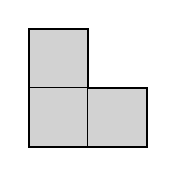
\begin{tikzpicture}[scale=0.75]

    \fill[gray!35] (0,0) rectangle (1,1);
    \fill[gray!35] (1,0) rectangle (2,1);
    \fill[gray!35] (0,1) rectangle (1,2);

    \draw[thick] (0,0) -- (2,0) -- (2,1) --
                 (1,1) -- (1,2) -- (0,2) -- cycle;

    \draw (1,0) -- (1,1);
    \draw (0,1) -- (1,1);

\end{tikzpicture}
\caption{An L-shaped tromino consisting of three unit squares.}
\label{fig:tromino}
\end{figure}

Suppose one square is removed from a $2^n\times2^n$  chessboard,
where $n\geq1$. Show that the remaining board can always be tiled completely
using L-shaped trominoes, irrespective of which square is removed.
\end{theorem}

\begin{proof}
Let $P(n)$ denote the statement
\[
P(n):\qquad
\text{Every $2^n\times2^n$ board with one square removed
can be tiled with L-shaped trominoes.}
\]
We shall prove $P(n)$ by mathematical induction.

\paragraph{Base case.}

For $n=1$, the board has size
\[
        2^1\times2^1=2\times2.
\]
It therefore consists of four unit squares. If any one square is
removed, the remaining three squares form exactly one L-shaped
tromino. Hence $P(1)$ is true.


\paragraph{Induction hypothesis.}

Suppose that $P(n)$ is true for some $n\geq1$. Thus we assume that
\emph{any} $2^n\times2^n$ board with one square removed can be tiled
completely using L-shaped trominoes.


\paragraph{Inductive step.}
We must show that $P(n+1)$ is true. Consider a
\[
        2^{n+1}\times2^{n+1}
\]
board from which one arbitrary square has been removed.

Divide the board into four equal quadrants. Each quadrant is a
$2^n\times2^n$ board. The missing square must lie in exactly one of
these four quadrants.

Without loss of generality, suppose that it lies in the top-left
quadrant, as illustrated in Figure~\ref{fig:tromino-induction}.

\begin{figure}[ht]
\centering

\begin{tikzpicture}[scale=0.70]

% An 8 x 8 board is used to illustrate the general construction.

% Shade the four quadrants lightly
\fill[gray!8]  (0,4) rectangle (4,8);
\fill[gray!16] (4,4) rectangle (8,8);
\fill[gray!16] (0,0) rectangle (4,4);
\fill[gray!8]  (4,0) rectangle (8,4);

% Grid
\draw[step=1,gray!55,thin] (0,0) grid (8,8);

% Outer boundary
\draw[very thick] (0,0) rectangle (8,8);

% Quadrant boundaries
\draw[very thick] (4,0) -- (4,8);
\draw[very thick] (0,4) -- (8,4);

% Original missing square in top-left quadrant
\fill[black] (1,6) rectangle (2,7);

% Central tromino:
% one square in top-right
\fill[gray!70] (4,4) rectangle (5,5);

% one square in bottom-left
\fill[gray!70] (3,3) rectangle (4,4);

% one square in bottom-right
\fill[gray!70] (4,3) rectangle (5,4);

% Borders of central tromino squares
\draw[thick] (4,4) rectangle (5,5);
\draw[thick] (3,3) rectangle (4,4);
\draw[thick] (4,3) rectangle (5,4);

% Quadrant labels
\node at (2,7.5) {\small Top-left};
\node at (6,7.5) {\small Top-right};
\node at (2,0.5) {\small Bottom-left};
\node at (6,0.5) {\small Bottom-right};

% Missing-square annotation
\draw[-{Latex},thick] (-0.5,6.5) -- (0.95,6.5);
\node[align=right] at (-1.6,6.5)
    {\small missing\\[-1mm]\small square};

% Central tromino annotation
\draw[-{Latex},thick] (9.1,3.7) -- (5.05,3.7);
\node[align=left] at (10.1,3.7)
    {\small central\\[-1mm]\small tromino};

\end{tikzpicture}
\caption{The $2^{n+1}\times2^{n+1}$ board is divided into four
$2^n\times2^n$ quadrants. The original missing square is shown in
black in the top-left quadrant. The shaded central L-shaped tromino
occupies one square in each of the other three quadrants.}
\label{fig:tromino-induction}
\end{figure}

Now comes the crucial observation. The top-left quadrant already has
one square missing. Place a single L-shaped tromino at the centre of
the board so that it occupies one central square in \emph{each of the
other three quadrants}.

After placing this central tromino:

\begin{enumerate}
    \item the top-left quadrant has exactly one square missing---the
          square that was originally removed;
    \item the top-right quadrant has exactly one square unavailable---the
          square occupied by the central tromino;
    \item the bottom-left quadrant similarly has exactly one square
          unavailable; and
    \item the bottom-right quadrant also has exactly one square
          unavailable.
\end{enumerate}

Thus we have transformed the original problem into four smaller
problems of precisely the form covered by the induction hypothesis.
Each quadrant is a $2^n\times2^n$ board with one square missing.

By the induction hypothesis, each of the four quadrants can therefore
be tiled completely with L-shaped trominoes. Together with the one
tromino that we have already placed at the centre, these tilings cover
the entire $2^{n+1}\times2^{n+1}$ board except for the originally
removed square.

Hence
\[
        P(n)\Longrightarrow P(n+1).
\]

Since $P(1)$ is true, the Principle of Mathematical Induction gives
\[
\boxed{
\text{Every $2^n\times2^n$ board with one square removed can be
tiled completely with L-shaped trominoes.}
}
\]
\end{proof}


\paragraph{Remarks.}
\begin{itemize}
  \item Induction proofs are especially useful for formulas involving sums, 
        products, inequalities, or divisibility.
  \item The induction hypothesis is a temporary assumption used to prove the 
        next case; it is not assumed globally.
  \item Strong induction is a variant where we assume the statement holds for 
        all integers up to $k$ and use this to prove it for $k+1$.
\end{itemize}

\subsection{Proofs of Equivalence}

Often in mathematics we want to prove a statement of the form
\[
P \;\Longleftrightarrow\; Q,
\]
which reads ``$P$ if and only if $Q$'' (abbreviated ``$P$ iff $Q$'').
This means both $P \Rightarrow Q$ and $Q \Rightarrow P$ hold. To prove such an
equivalence, we usually split the work into two parts:

\begin{enumerate}
\item Prove the \emph{forward implication} $P \Rightarrow Q$.
\item Prove the \emph{reverse implication} $Q \Rightarrow P$.
\end{enumerate}

Equivalences require a special discussion because sometimes the two directions may use very different arguments. Consider the following examples.


\begin{theorem}
An integer $n$ is even $\;\Longleftrightarrow\;$ $n^2$ is even.
\end{theorem}
\begin{proof}
\textbf{($\Rightarrow$)} Suppose $n$ is even, say $n=2k$. Then
$n^2=(2k)^2=4k^2=2(2k^2)$ is even.

\textbf{($\Leftarrow$)} Conversely, suppose $n^2$ is even. If $n$ were odd,
say $n=2k+1$, then $n^2=(2k+1)^2=4k^2+4k+1=2(2k^2+2k)+1$, which is odd —
a contradiction. Hence $n$ must be even.
\end{proof}


\begin{theorem}
The Well-Ordering Principle for $\mathbb N$ (Section \ref{sec:well-ordering})  and the Principle of Mathematical Induction 
 are equivalent.
\end{theorem}

\begin{proof}

\noindent
\textbf{($\Rightarrow$) Well-ordering implies mathematical induction}

Assume the Well-Ordering Principle.

Suppose that $P(n)$ is a statement satisfying
        $P(0)$  and $P(n)\Longrightarrow P(n+1) \text{ for every }n\in\mathbb N.$

We want to prove that $P(n)$ is true for every $n\in\mathbb N$.

Suppose, to the contrary, that this is not so. Then there is at least
one natural number for which $P(n)$ is false. Consider the set
\[
        C=\{n\in\mathbb N:P(n)\text{ is false}\}.
\]

Our assumption says that $C$ is non-empty. By the Well-Ordering
Principle, $C$ therefore has a least element. Call it $m$.

Since $P(0)$ is true,
\[
        m\neq0.
\]
Hence $m>0$, and therefore $m-1\in\mathbb N$.

Since $m$ is the \emph{least} member of $C$, $m-1$ cannot belong to
$C$. Consequently,
\[
        P(m-1)
\]
must be true.

But the inductive condition tells us that
\[
        P(m-1)\Longrightarrow P(m).
\]
Therefore $P(m)$ is true.

This contradicts the fact that $m\in C$, which says that $P(m)$ is
false.

Hence $C$ must be empty. There are no counterexamples, and therefore
\[
        P(n)\text{ is true for every }n\in\mathbb N.
\]

Thus the Well-Ordering Principle implies the Principle of Mathematical
Induction.

Notice the idea behind this argument. If induction were to fail, there
would have to be a \emph{first} place where it fails. But if the
statement is true immediately before that first failure, the inductive
step says that it must also be true at the supposed first failure.
This is impossible.

\noindent
\textbf{($\Leftarrow$)Mathematical induction implies well-ordering}

Now assume the Principle of Mathematical Induction.

We want to prove the Well-Ordering Principle. Suppose, to the contrary,
that it is false. Then there exists some non-empty set
\[
        S\subseteq\mathbb N
\]
that has no least element.

We shall use induction to show that no natural number can belong to
$S$. This will contradict the assumption that $S$ is non-empty.

Define the statement
\[
        P(n):
        \qquad
        0,1,\ldots,n\notin S.
\]

In other words, $P(n)$ says that none of the natural numbers from $0$
through $n$ belongs to $S$.

\paragraph{Base case.}
We claim that
\[
        0\notin S.
\]
For if $0\in S$, then $0$ would automatically be the least element of
$S$, since no natural number is smaller than $0$. This contradicts our
assumption that $S$ has no least element.

Therefore $P(0)$ is true.

\paragraph{Inductive step.}
Suppose $P(n)$ is true. Thus
\[
        0,1,\ldots,n\notin S.
\]

We must show that $P(n+1)$ is true.

Suppose instead that
\[
        n+1\in S.
\]
Since none of
\[
        0,1,\ldots,n
\]
belongs to $S$, there can be no element of $S$ smaller than $n+1$.
Therefore $n+1$ would be the least element of $S$.

But we assumed that $S$ has no least element. Hence
\[
        n+1\notin S.
\]

Thus
\[
        P(n)\Longrightarrow P(n+1).
\]

By the Principle of Mathematical Induction, $P(n)$ is true for every
$n\in\mathbb N$. Hence
\[
        n\notin S
        \qquad\text{for every }n\in\mathbb N.
\]

Therefore
\[
        S=\emptyset.
\]

But this contradicts our assumption that $S$ is non-empty. Consequently,
every non-empty subset of $\mathbb N$ must have a least element.

Thus mathematical induction implies the Well-Ordering Principle.
\end{proof}

\paragraph{Remark.} The two principles describe the same fundamental structure of the
natural numbers from different viewpoints.

The Well-Ordering Principle looks \emph{backwards}: if something happens
somewhere among the natural numbers, there must be a \emph{first} place
where it happens.

Mathematical induction looks \emph{forwards}: start at $0$, and if a
property can always be carried from $n$ to $n+1$, then it propagates
through all the natural numbers.

This also explains why the method of the \emph{smallest counterexample}
is so closely related to induction. To prove that $P(n)$ holds for all
$n$, suppose that counterexamples exist. Well-ordering gives us a
smallest counterexample. We then use what is true for smaller numbers
to show that this supposed smallest counterexample cannot actually be
one.

Thus induction, well-ordering, and proofs using a smallest
counterexample are not unrelated tricks. They are different
manifestations of the same underlying structure of the natural numbers.


%%%%%%%%%%%
\subsection{Equivalence of Several Statements: Circular Implication}
\label{sec:circular-implication}

We have seen that to prove two statements $P$ and $Q$ equivalent, we
prove both directions
\[
        P\Longrightarrow Q
        \qquad\text{and}\qquad
        Q\Longrightarrow P.
\]

What should we do if we want to prove that three statements $P$, $Q$,
and $R$ are all equivalent?

One possibility would be to prove every implication separately:
\[
\begin{array}{ccc}
P\Rightarrow Q, & P\Rightarrow R, &
Q\Rightarrow P,\\
Q\Rightarrow R, & R\Rightarrow P, &
R\Rightarrow Q.
\end{array}
\]
But this is unnecessary. It is enough to prove the three implications
\[
        P\Longrightarrow Q,\qquad
        Q\Longrightarrow R,\qquad
        R\Longrightarrow P.
\]
These form a \emph{circular implication}:
\[
\boxed{
        P\Longrightarrow Q
        \Longrightarrow R
        \Longrightarrow P.
}
\]

Why is this sufficient? For example, $P\Rightarrow R$ follows by
combining
\[
        P\Rightarrow Q\Rightarrow R,
\]
while $Q\Rightarrow P$ follows from
\[
        Q\Rightarrow R\Rightarrow P.
\]
Similarly,
\[
        R\Rightarrow P\Rightarrow Q
\]
gives $R\Rightarrow Q$. Thus every statement implies every other
statement, and hence
\[
        P\Longleftrightarrow Q\Longleftrightarrow R.
\]

This method is particularly useful when different links in the circle
are naturally proved in different ways.


\subsubsection*{Example 1: Three characterizations involving even integers}

Let $n\in\mathbb Z$. Consider the following three statements:
\[
\begin{aligned}
P &: \quad n \text{ is even},\\
Q &: \quad n^2 \text{ is even},\\
R &: \quad n^2+2n \text{ is even}.
\end{aligned}
\]

We shall prove that
\[
        P\Longleftrightarrow Q\Longleftrightarrow R
\]
by establishing the circular implication
\[
        P\Longrightarrow Q
        \Longrightarrow R
        \Longrightarrow P.
\]

\paragraph{$P\Rightarrow Q$.}
Suppose $n$ is even. Then
\[
        n=2k
\]
for some $k\in\mathbb Z$. Therefore
\[
        n^2=(2k)^2=4k^2=2(2k^2),
\]
so $n^2$ is even. Hence
\[
        P\Longrightarrow Q.
\]

\paragraph{$Q\Rightarrow R$.}
Suppose $n^2$ is even. Since $2n$ is also even,
\[
        n^2+2n
\]
is the sum of two even integers and is therefore even. Hence
\[
        Q\Longrightarrow R.
\]

\paragraph{$R\Rightarrow P$.}
For this direction it is convenient to prove the contrapositive.
Suppose $n$ is odd. Then $n+2$ is also odd. Since
\[
        n^2+2n=n(n+2),
\]
and the product of two odd integers is odd, $n^2+2n$ is odd.

Thus
\[
        n\text{ odd}
        \Longrightarrow
        n^2+2n\text{ odd}.
\]
Taking the contrapositive,
\[
        n^2+2n\text{ even}
        \Longrightarrow
        n\text{ even}.
\]
Hence
\[
        R\Longrightarrow P.
\]

We have therefore completed the circle:
\[
\boxed{
n\text{ even}
\Longrightarrow
n^2\text{ even}
\Longrightarrow
n^2+2n\text{ even}
\Longrightarrow
n\text{ even}.
}
\]

Consequently,
\[
\boxed{
n\text{ is even}
\quad\Longleftrightarrow\quad
n^2\text{ is even}
\quad\Longleftrightarrow\quad
n^2+2n\text{ is even}.
}
\]

Notice that the three parts of the proof need not use the same proof
technique. The first implication follows directly from the definition
of an even integer, the second uses the fact that the sum of two even
integers is even, and the third is most naturally proved by
contrapositive. Circular implication tells us how these separate
arguments can be assembled into a single proof of equivalence.


\subsubsection*{Example 2: Divisibility by $6$}

Here is a slightly more substantial example. Let $n\in\mathbb Z$ and
consider
\[
\begin{aligned}
P &: \quad 6\mid n,\\
Q &: \quad 2\mid n\text{ and }3\mid n,\\
R &: \quad 6\mid n^2.
\end{aligned}
\]

We shall again prove
\[
        P\Longleftrightarrow Q\Longleftrightarrow R
\]
by establishing
\[
        P\Longrightarrow Q
        \Longrightarrow R
        \Longrightarrow P.
\]

\paragraph{$P\Rightarrow Q$.}
Suppose $6\mid n$. Then
\[
        n=6k
\]
for some $k\in\mathbb Z$. But
\[
        n=2(3k)
        \qquad\text{and}\qquad
        n=3(2k).
\]
Therefore
\[
        2\mid n
        \qquad\text{and}\qquad
        3\mid n.
\]
Hence
\[
        P\Longrightarrow Q.
\]

\paragraph{$Q\Rightarrow R$.}
Suppose
\[
        2\mid n
        \qquad\text{and}\qquad
        3\mid n.
\]
Since $2$ and $3$ are relatively prime, this implies
\[
        6\mid n.
\]
Thus $n=6k$ for some $k\in\mathbb Z$, and consequently
\[
        n^2=36k^2=6(6k^2).
\]
Hence
\[
        6\mid n^2,
\]
and therefore
\[
        Q\Longrightarrow R.
\]

\paragraph{$R\Rightarrow P$.}
Suppose
\[
        6\mid n^2.
\]
Then
\[
        2\mid n^2
        \qquad\text{and}\qquad
        3\mid n^2.
\]

We use the fact that if $p$ is prime and
\[
        p\mid a^2,
\]
then
\[
        p\mid a.
\]
Since both $2$ and $3$ are prime, it follows that
\[
        2\mid n
        \qquad\text{and}\qquad
        3\mid n.
\]
Since $2$ and $3$ are relatively prime,
\[
        6\mid n.
\]
Therefore
\[
        R\Longrightarrow P.
\]

We have again completed the circle:
\[
\boxed{
6\mid n
\Longrightarrow
(2\mid n\text{ and }3\mid n)
\Longrightarrow
6\mid n^2
\Longrightarrow
6\mid n.
}
\]

Thus
\[
\boxed{
6\mid n
\quad\Longleftrightarrow\quad
(2\mid n\text{ and }3\mid n)
\quad\Longleftrightarrow\quad
6\mid n^2.
}
\]

This example requires two elementary facts about divisibility:
\[
\gcd(2,3)=1
\quad\Longrightarrow\quad
(2\mid n\text{ and }3\mid n)\Longrightarrow6\mid n,
\]
and, for a prime $p$,
\[
        p\mid n^2\Longrightarrow p\mid n.
\]
The latter is a consequence of Euclid's Lemma. 


\subsubsection*{Circular implication in general}

The same idea extends beyond three statements. Suppose we want to show
that
\[
        P_1,P_2,\ldots,P_k
\]
are all equivalent. It is sufficient to establish the cycle
\[
\boxed{
P_1\Longrightarrow P_2
\Longrightarrow P_3
\Longrightarrow\cdots
\Longrightarrow P_k
\Longrightarrow P_1.
}
\]

Starting from any one of these statements, we can follow the arrows
around the circle to reach any of the others. Hence every statement
implies every other statement.

This can substantially reduce the amount of work required. If we tried
to prove every directed implication separately, there would be
\[
        k(k-1)
\]
implications to prove. A circular proof requires only
\[
        k
\]
implications.

The important point, however, is not merely that circular implication
saves work. It allows us to choose the \emph{most natural direction}
between successive statements. One implication may have a simple
direct proof, another may follow from an already established theorem,
and another may be easiest to prove by contrapositive. The resulting
circle then establishes the equivalence of all the statements.


%%%%%%%%%%%%

%\paragraph{Discussion.}
%When faced with an equivalence, it is often useful to remember that
%``$P \Longleftrightarrow Q$'' is logically the same as
%``$(P \Rightarrow Q) \land (Q \Rightarrow P)$.''
%It is also common to use \emph{contrapositive arguments} in one or both directions.
%\subsection{Proof by Induction}
%Induction proves infinitely many cases with two finite checks. Think of a staircase: show you can step onto the first stair (base case) and that from any stair you can step to the next (inductive step). Then you can reach all stairs.
%
%\begin{theorem}\label{thm:sum}
%For all \(n\ge 1\),
%\[
%1+2+\cdots+n=\frac{n(n+1)}{2}.
%\]
%\end{theorem}
%\begin{proof}
%\textbf{Base case:} \(n=1\) gives \(1=\tfrac{1\cdot2}{2}\). \\
%\textbf{Inductive step:} Assume true for \(n=k\):
%\(
%1+\cdots+k=\frac{k(k+1)}{2}.
%\)
%Then
%\[
%1+\cdots+k+(k+1)=\frac{k(k+1)}{2}+(k+1)=\frac{(k+1)(k+2)}{2}.
%\]
%Thus true for \(k{+}1\). By induction, true for all \(n\ge1\).
%\end{proof}

%\paragraph{Tips for induction.}
%(1) State the predicate \(P(n)\) explicitly. (2) In the step, begin with the left-hand side for \(n{+}1\) and \emph{inject} the hypothesis where it naturally matches. (3) Strong induction is the variant where you assume all cases up to \(k\) to prove \(k{+}1\).
%
%\begin{figure}[h]
%\centering
%\begin{tikzpicture}[x=1.2cm,y=0.9cm, every node/.style={font=\small}]
%  % stairs
%  \foreach \i in {0,...,5}{
%    \draw (0,\i) -- (5-\i,\i);
%    \draw (5-\i,\i) -- (5-\i,\i+1);
%  }
%  % labels
%  \node at (0.3,0.4) {$n=1$};
%  \node at (1.3,1.4) {$n=2$};
%  \node at (2.3,2.4) {$n=3$};
%  \node at (3.3,3.4) {$\cdots$};
%  % arrows
%  \draw[-{Latex}] (-0.8,0.5) -- (0,0.5) node[midway, above] {Base case};
%  \draw[-{Latex}] (0.8,0.9) -- (1,1.1);
%  \draw[-{Latex}] (1.8,1.9) -- (2,2.1);
%  \draw[-{Latex}] (2.8,2.9) -- (3,3.1);
%  \node[align=left] at (4.3,4.7) {Inductive step\\ $n\Rightarrow n{+}1$};
%\end{tikzpicture}
%\caption{Induction as a staircase: base case + step implies all cases.}
%\end{figure}
%
%
%
%
%\section{Further Worked Examples (Variety)}
%\paragraph{Direct (case split).} Let \(\operatorname{MAX}(a,b)=\max\{a,b\}\). If \(a>c\) and \(b>c\), then \(\operatorname{MAX}(a,b)-c>0\). \emph{Proof:} If \(a\ge b\), then \(\operatorname{MAX}=a>c\Rightarrow a-c>0\). If \(b>a\), similarly \(b-c>0\).
%
%\paragraph{Contradiction (infinitely many primes).} Assume only finitely many primes \(p_1,\dots,p_n\). Consider \(k=p_1\cdots p_n+1\). Any prime divisor of \(k\) differs from each \(p_i\), contradiction.
%
%\paragraph{Induction (divisibility).} Show \(7\mid (8^n-1)\) for all \(n\ge1\). Base \(n=1\): \(8-1=7\). Step: \(8^{k+1}-1=8(8^k-1)+7\) is divisible by \(7\) if \(8^k-1\) is.
%
%\paragraph{Contrapositive (parity).} If \(x^2\) is even, then \(x\) is even. Contrapositive: if \(x\) is odd, \(x^2\) is odd (proved above).

\subsection{Conclusion}
There is no single ``best'' technique; experienced problem solvers try viewpoints. If definitions seem aligned, push a direct proof. If ``not \(Q\)’’ feels structured, flip to a contrapositive. If a statement ranges over integers, try induction. If you suspect a claim is too strong, hunt a counter-example. And whenever “assuming the opposite’’ quickly generates an impossibility, contradiction is often the sharpest tool.

\section*{Problems}

\begin{enumerate}

% -------------------------
% Truth Tables
% -------------------------
\item \textbf{Truth Tables}
  \begin{enumerate}
    \item Construct the truth table for $(p \land q) \lor (\lnot r)$.
    \item Verify by a truth table that $(p \Rightarrow r) \land (q \Rightarrow r)$
          is equivalent to $(p \lor q) \Rightarrow r$.
    \item Determine whether $(p \Rightarrow q) \Rightarrow r$ and
          $p \Rightarrow (q \Rightarrow r)$ are equivalent.
    \item Show by truth table that $p \lor (q \land r)$ is not equivalent to
          $(p \lor q) \land (p \lor r)$.
  \end{enumerate}

% -------------------------
% Three-variable / multi-variable Logic
% -------------------------
\item \textbf{Three-variable Logic}
  \begin{enumerate}
    \item Construct the truth table for $(p \oplus q) \oplus r$ and check whether it is associative.
    \item Verify that $\lnot(p \land q \land r)$ is equivalent to $\lnot p \lor \lnot q \lor \lnot r$.
    \item Show that $(p \Rightarrow q) \land (q \Rightarrow r)$ does not imply $(p \Rightarrow r)$ by giving a truth table.
    \item Identify all assignments of $p,q,r$ for which $(p \lor q) \Rightarrow (q \lor r)$ is false.
  \end{enumerate}

% -------------------------
% Vacuous Truth
% -------------------------
\item \textbf{Vacuous Truth}
  \begin{enumerate}
    \item State a universally quantified claim about an empty set and explain why it is true.
    \item Explain why the statement ``If $n$ is an integer with $n^2=-1$, then $n$ is prime'' is vacuously true.
    \item Let $A=\varnothing$. Prove that ``For all $x\in A$, $x^2=0$'' is vacuously true.
    \item Formulate a vacuous truth involving divisibility (e.g.\ ``All integers divisible by both 2 and 3 and equal to 5 are even''), and justify why it is vacuously true.
  \end{enumerate}

% -------------------------
% Explicit Construction
% -------------------------
\item \textbf{Proof by Explicit Construction}
  \begin{enumerate}
    \item Find integers $x,y$ such that $17x+29y=1$.
    \item Exhibit an explicit Pythagorean triple different from $(3,4,5)$ and $(5,12,13)$.
    \item Construct a rational number between $\tfrac{7}{9}$ and $\tfrac{8}{9}$.
    \item Show by construction that there exists an integer solution to $12x+18y=6$.
  \end{enumerate}

% -------------------------
% Counter-Example
% -------------------------
\item \textbf{Proof by Counter-Example}
  \begin{enumerate}
    \item Disprove: ``For all integers $n$, $n^2-n+41$ is prime.''
    \item Disprove: ``For all integers $n$, $n^3+2$ is prime.''
    \item Disprove: ``Every integer greater than 2 is the sum of two primes.'' (Give a counterexample.)
    \item Find a counterexample to: ``If $a$ divides $bc$, then $a$ divides $b$.'' 
  \end{enumerate}

% -------------------------
% Direct Proof
% -------------------------
\item \textbf{Direct Proof}
  \begin{enumerate}
    \item Prove that the product of two even integers is even.
    \item Prove that if $a$ is divisible by 12 and $b$ is divisible by 6, then $a+b$ is divisible by 6.
    \item Show directly that if $n$ is a multiple of 4, then $n^2$ is a multiple of 16.
    \item Prove directly that if $a\equiv b \pmod{m}$ and $c\equiv d \pmod{m}$, then $a+c \equiv b+d \pmod{m}$.
  \end{enumerate}

% -------------------------
% Contradiction
% -------------------------
\item \textbf{Proof by Contradiction}
  \begin{enumerate}
    \item Prove by contradiction that $\sqrt{7}$ is irrational.
    \item Show by contradiction that there is no integer solution to $2x=2y+1$.
    \item Prove by contradiction that there are infinitely many primes congruent to 1 modulo 4.
    \item Prove by contradiction that $\sqrt[3]{2}$ is irrational.
  \end{enumerate}

% -------------------------
% Contrapositive
% -------------------------
\item \textbf{Proof by Contrapositive}
  \begin{enumerate}
    \item Prove: If $n^2$ is divisible by 9, then $n$ is divisible by 3.
    \item Prove: If $ab$ is even, then at least one of $a$ or $b$ is even.
    \item Prove: If $n^2$ is divisible by 8, then $n$ is divisible by 2.
    \item Prove: If $x^2$ is divisible by 12, then $x$ is divisible by 6.
  \end{enumerate}

% -------------------------
% Pigeonhole
% -------------------------
\item \textbf{Proof by the Pigeonhole Principle}
  \begin{enumerate}
    \item Show that among any 8 integers, two leave the same remainder modulo 7.
    \item Prove that in a group of 32 people, at least two share the same day of the month for their birthday.
    \item Show that in any set of 6 integers, at least three must have the same parity.
    \item Prove that in any group of 367 people, at least two have the same exact birthday (ignoring leap years).
  \end{enumerate}

% -------------------------
% Exhaustion
% -------------------------
\item \textbf{Proof by Exhaustion of Cases}
  \begin{enumerate}
    \item Prove that the cube of any integer is congruent to $-1,0,$ or $1$ modulo 7.
    \item Show that if $n$ is an integer, then $n^2 \equiv 0,1,4 \pmod{5}$.
    \item By checking cases, show that for any integer $n$, $n^2-n$ is even.
    \item Prove by exhaustion of parities that the product of two consecutive integers is even.
  \end{enumerate}

% -------------------------
% Equivalence
% -------------------------
\item \textbf{Proofs of Equivalence}
  \begin{enumerate}
    \item Prove that $n$ is divisible by 2 if and only if $n^2$ is divisible by 4.
    \item Prove that $a \equiv b \pmod{n}$ if and only if $a$ and $b$ leave the same remainder when divided by $n$.
    \item Prove that an integer $n$ is divisible by 11 if and only if the alternating sum of its digits is divisible by 11.
    \item Prove that $a$ and $b$ are both even if and only if $a+b$ is even and $a-b$ is even.
  \end{enumerate}
  
\item \textbf{Proof by Induction}
\begin{enumerate}

      \item  Find the fallacy in the following proof by {\bf PMI}. \newline
        {\bf Theorem}
        Given any collection of $n$ blonde girls. If at least one of the 
        girls has blue eyes, then all $n$ of them have blue eyes. \newline
        \begin{proof}
        The statement is obviously true for $n = 1$. The step from $k$ to
        $k+1$ can be illustrated by going from $n = 3$ to $n = 4$. Assume,
        therefore, that the statement is true for $n = 3$ and let
        $G_1,G_2,G_3,G_4$ be four blonde girls, at least one of which,
        say $G_1$, has blue eyes.  Taking $G_1,G_2,$ and $G_3$ together
        and using the fact that the statement is true when $n = 3$, we find
        that $G_2$ and $G_3$ also have blue eyes. Repeating the process
        with $G_1,G_2$ and $G_4$, we find that $G_4$ has blue eyes. Thus
        all four have blue eyes. A similar argument allows us to make
        the step from $k$ to $k+1$ in general.
        \end{proof} \newline
        {\bf Corollary.} All blonde girls have blue eyes. \newline
        \begin{proof}
        Since there exists at least one blonde girl with blue eyes, we
        can apply the foregoing result to the collection consisting
        of all blonde girls.
        \end{proof}  \newline
        {\em Note:} This example is from G. P\'{o}lya, who suggests that the reader may want to test the validity of the statement by experiment.
        
        \item Suban announces to the QRMT class:

               ``There will be a surprise test next week. You will not know in advance on which day it will be held.''

One student in the class reasons as follows, by induction on $n = 5 - k$:
\begin{itemize}
	\item	The test cannot be on Friday (the last working day of the week, $k=5,n=0$), because if it hasn’t happened before then, the class would know it must be on Friday — and so it would not be a surprise.
	 \item	Similarly, the test cannot be on Thursday, because if it hasn’t happened before then, and Friday has already been ruled out, the class would know it must be on Thursday — and so it would not be a surprise.
	\item	Continuing this reasoning backwards, the test cannot be on Wednesday, Tuesday, or Monday either.
	\item	Therefore, the teacher cannot give a surprise test at all!
\end{itemize}
Yet, when Suban gives the test on Wednesday, the students are indeed surprised. Identify the flaw in the student's reasoning.

    
      \item Prove by induction that for all integers $n \geq 1$,
      \[
      1^2 + 2^2 + 3^2 + \cdots + n^2 = \frac{n(n+1)(2n+1)}{6}.
      \]
   

      \item Show by induction that $7^n - 1$ is divisible by $6$ for all integers $n \geq 1$.
      \item Prove that for all $n \geq 1$, $n^3 - n$ is divisible by $6$.

      \item Prove that for all integers $n \geq 4$, 
      \[
      n! > 2^n.
      \]
      \item Show that for all integers $n \geq 1$,
      \[
      3^n \geq n^3.
      \]


      \item Prove using strong induction that every integer $n > 1$ can be written as a product of prime numbers.
      \item A tiling problem: Prove by strong induction that any $2^n \times 2^n$ chessboard with one square removed can be covered completely by L-shaped trominoes (three-square pieces).
   
\end{enumerate}

\end{enumerate}

